
\documentclass[12pt]{article}
\usepackage[margin=1in]{geometry}

% \usepackage[margin=1.5in]{geometry} % Please keep the margins at 1.5 so that there is space for grader comments.
\PassOptionsToPackage{export}{adjustbox}
\usepackage{amsmath, hyperref, subfig, amsthm,amssymb,hyperref,amsfonts,framed,tabto,listings, dirtytalk, graphicx, tikz, pgf, adjustbox, physics}
\usepackage{enumitem}
% \usepackage[export]{adjustbox}
% \usetikzlibrary{arrows}

\newcommand{\R}{\mathbf{R}}  
\newcommand{\Z}{\mathbf{Z}}
\newcommand{\N}{\mathbf{N}}
\newcommand{\Q}{\mathbf{Q}}
\newcommand{\overbar}[1]{\mkern 1.5mu\overline{\mkern-1.5mu#1\mkern-1.5mu}\mkern 1.5mu}
% \newcommand{\sbt}{\,\begin{picture}(-1,1)(-1,-3)\circle*{3}\end{picture}\ }
% \graphicspath{.}


\newenvironment{theorem}[2][Theorem]{\begin{trivlist}
\item[\hskip \labelsep {\bfseries #1}\hskip \labelsep {\bfseries #2.}]}{\end{trivlist}}
% \newenvironment{solution}{\begin{proof}[Solution]}{\end{proof}}
\author{Ben Zuckier}
\date{\vspace{-3ex}}
\title{\vspace{-2.5cm}Gravity from a Rod Pendulum}
\begin{document}
\maketitle

\vspace{-1cm}

\section{Abstract}
    In this experiment, a physical pendulum is used to calculate the local value for gravity, $g$. High precision and accuracy are the goal, so certain careful corrections will be made and great care will be taken. The author chose to use a ``rod pendulum'', a pendulum made from a suspended rod -- i.e. it has no ``bob''. This will simplify some calculations, as will be shown. The final value for gravity is $g=9.912 \pm .004$

    Accuracy $a=0.011$ and precision $p=0.0004$.

\section{Text}
    \begin{enumerate}[label=(\alph*)]
        \item Introduction:\\
        A rod pendulum is used. The equation for the period of a rod pendulum is\\ $T = 2\pi\sqrt{\frac{\frac{1}{3}mL^2}{mg\frac{L}{2}}}$ -- keeping in mind that the moment of inertia for a rod suspended from one end is $I=\frac{1}{3}mL^2$ -- which amazingly simplifies to $T=2\pi \sqrt{\frac{2L}{3g}}$. As such the mass and radius of the rod have no bearing on the period! If we rearrange for $g$ we find \[
            g = \left(\frac{8\pi^2}{3}\right) \frac{L}{T^2}    
        \]
        \item Materials and Methods:\\
        A steel rod was attached to a small hinge and attached to the ceiling, such that it could swing freely. The hinge was lubricated very well with silicone lubricant. The length of the rod from the pivot point was measured using a millimeter marked measuring tape, and the thickness was measured with calipers with markings every half ``thou'', or 1/2000 of an inch. Care was taken to ensure that there was no bounce or wobble from the setup and that everything was centered.

        The following is 2 pictures of the setup, and an \href{https://photos.app.goo.gl/3uDxVGnjeVLDAJ4e7}{album} containing a video and more photos is linked below: \footnote{\url{https://photos.app.goo.gl/3uDxVGnjeVLDAJ4e7}}\\

        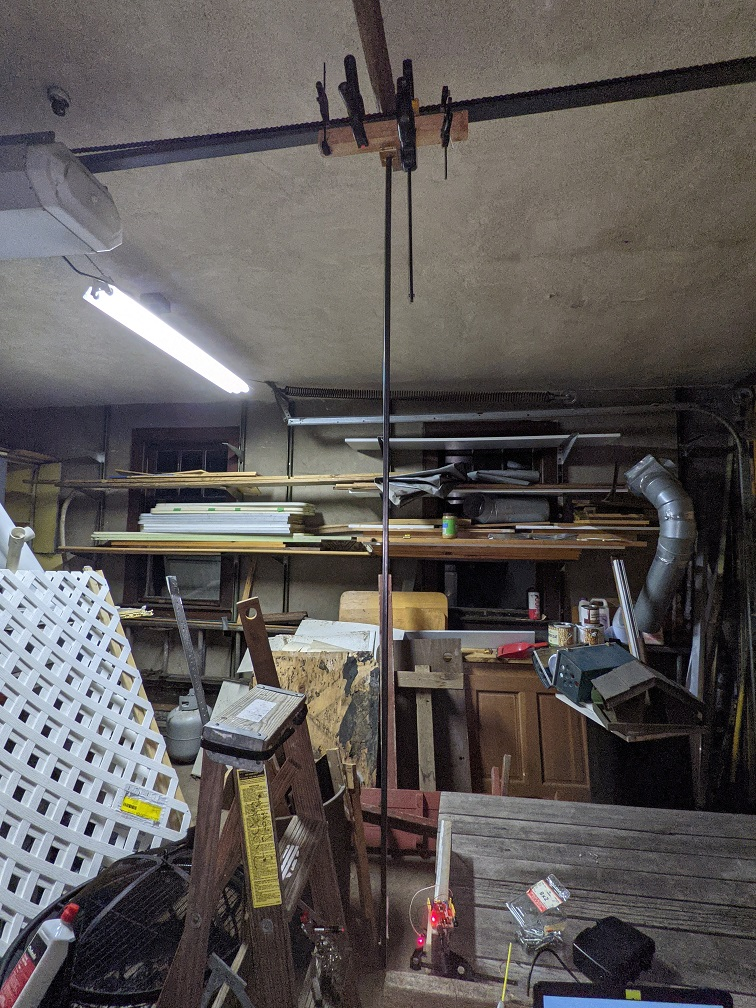
\includegraphics[width=3in]{whole.jpg}
        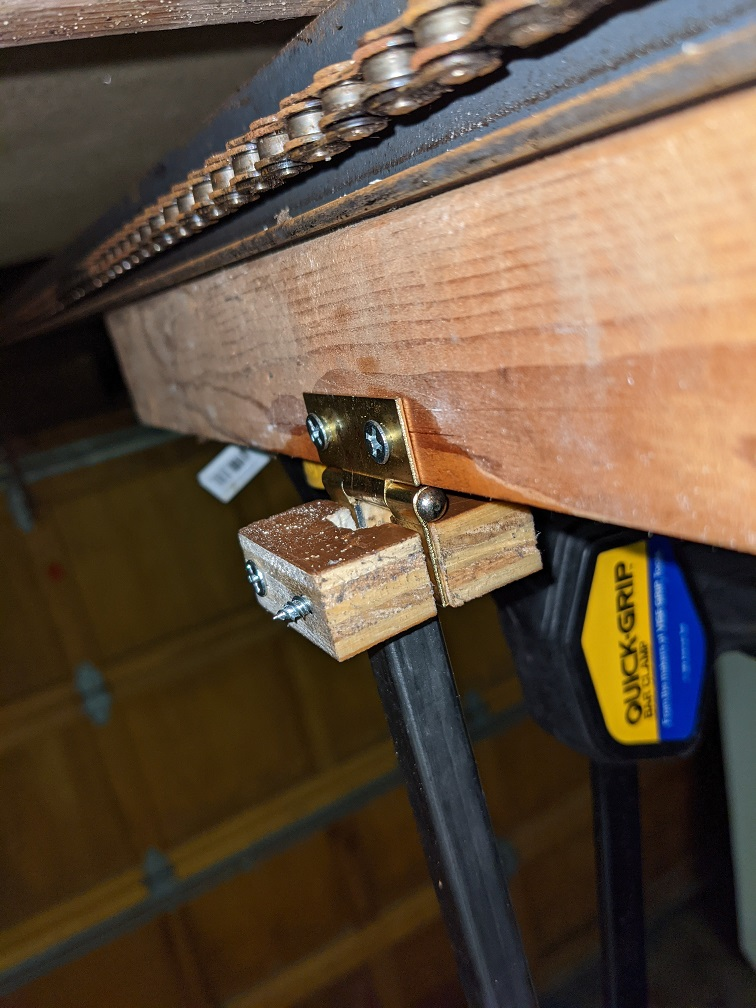
\includegraphics[width=3in]{hinge.jpg}\\

        An LED was wired backwards to the input pin of an Arduino microcontroller, such that it would behave as a photodiode, i.e. a voltage would be generated across its leads when light is applied to the diode. A laser was shone on the diode such that the pendulum would intersect its path and thereby interrupt the light going to the photodiode and the microcontroller could record this change in luminance and the period could be derived. A program was written in Python which recorded these values and well as the computer time to the nearest millisecond.\\
        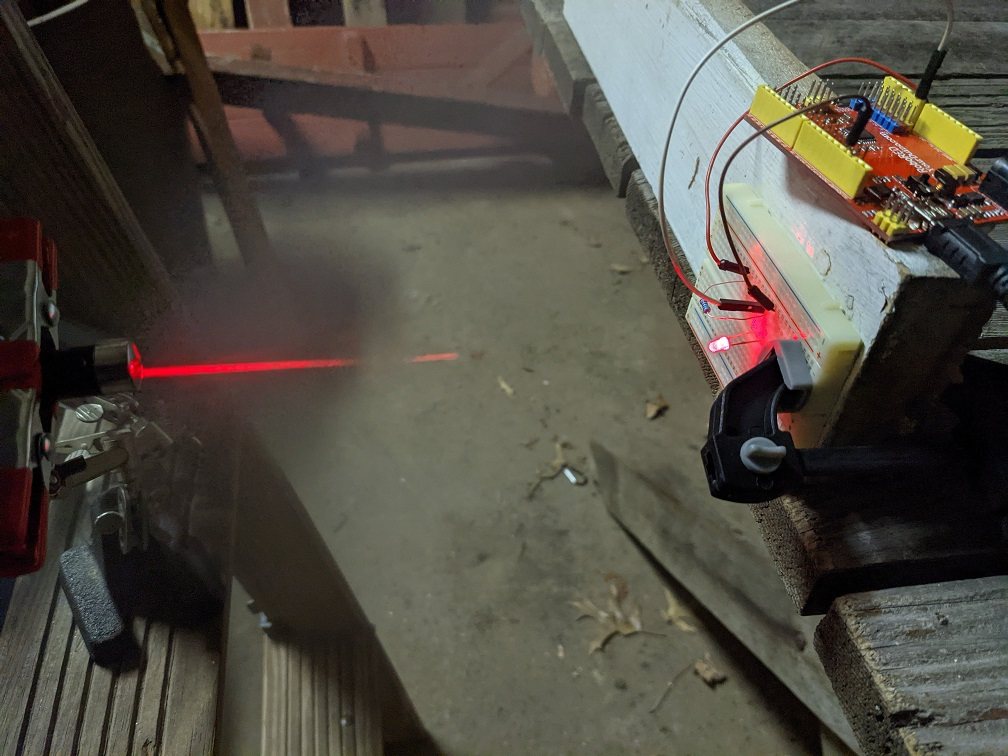
\includegraphics[width=4in]{las.jpg}\\

        Later, a program was used to clean messy data (values way out of range) and then to find the time between when the luminance first drops to when it goes high at the end of the cycle -- the falling edge and then the rising edge. This ensures that it's always calculating from the same ``side'' of the pendulum, as the pendulum has width, and therefore at the exact same point in the oscillation. This was done for every oscillation. This gives extremely precise results, to the nearest millisecond.
        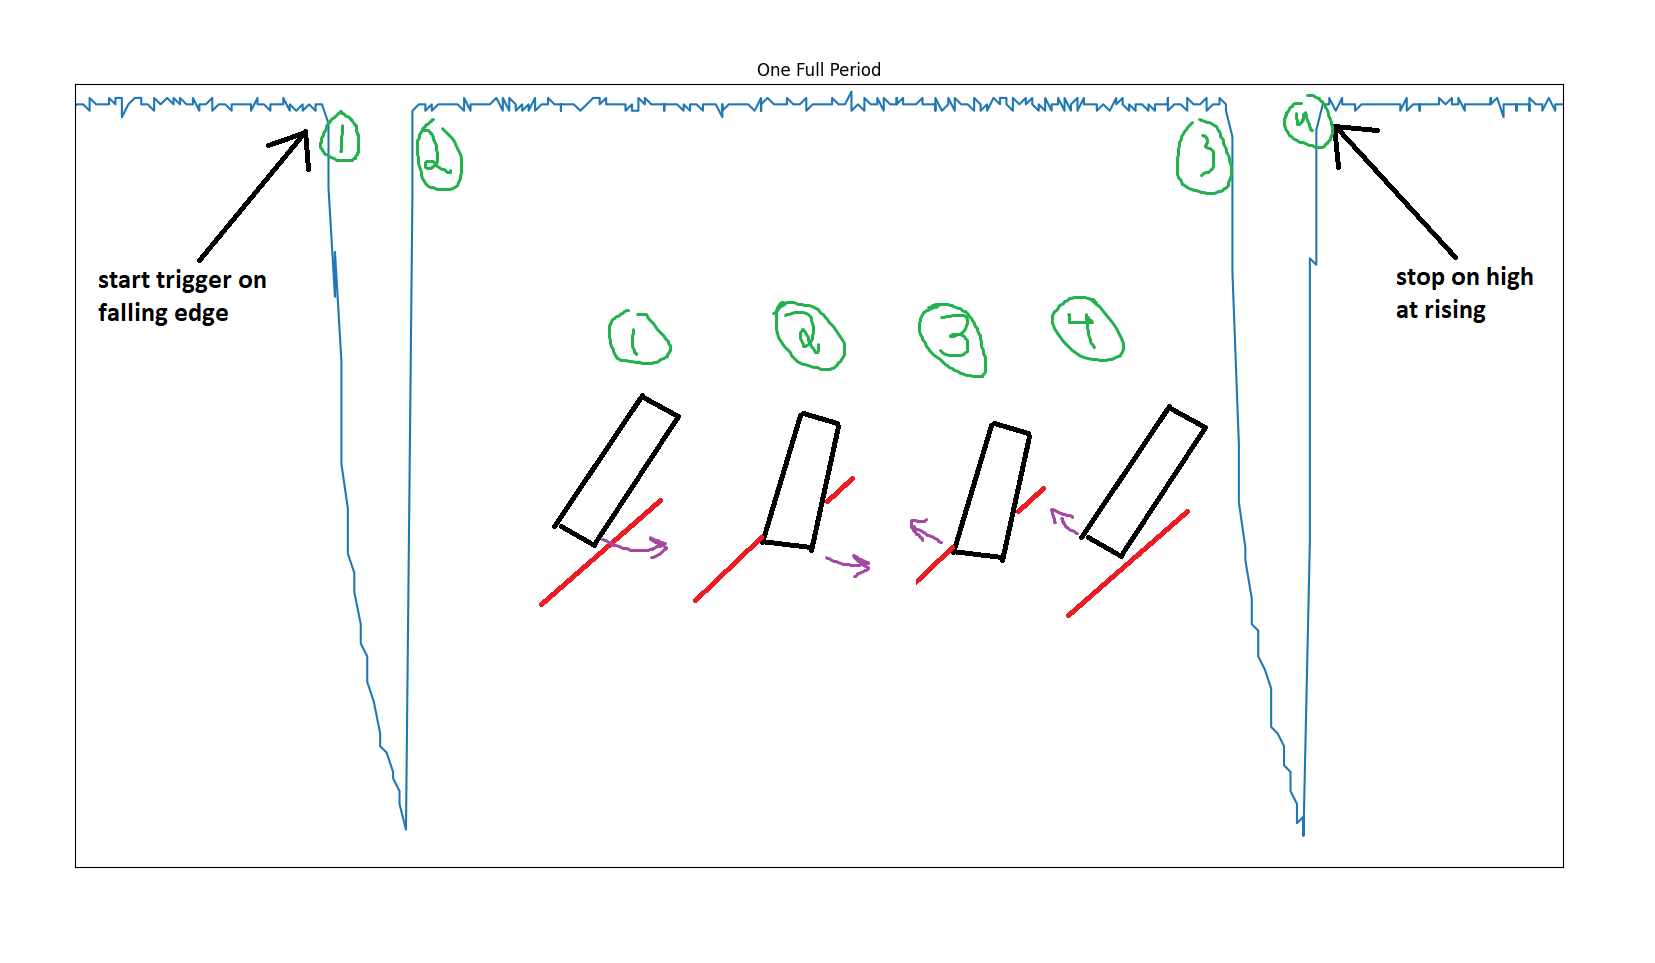
\includegraphics[width=6in]{period.png}\\

        Four runs were performed, each with 79 to 85 full periods. The oscillations were started at $20^\circ$ and stopped at $5^\circ$. This will be used to correct for ``finite amplitude''.

        Here is a table of the dimensions of the pendulum. As noted, the mass and radius is irrelevant for this setup.\\

        \begin{center}
            \begin{tabular}{ ||c||c|c|| } 
                \hline
                \textbf{Item} & Value & Uncertainty \\ 
                \hline
                \textbf{Rod Length} (cm) & 167.6 & .05\\ 
                \textbf{Rod Width} (cm) & 1.28 & .001\\ 
                \textbf{Rod Thickness} (cm) & 0.167 & .0006\\ 
                \textbf{Rod Weight} (kg) & 1.124 & .0005\\ 
                \textbf{String} & N/A & N/A\\ 
                \hline
            \end{tabular}
        \end{center}
        % \includegraphics[width=4in]{dim.png}\\

        \item Results and Discussion:\\
            The average of the 80 or so oscillations per each run were taken and an average of those was taken. The angle is finite so we have to correct using the perturbation expansion. Since the angle started at 20 degrees and ended at 5 degrees we will take the average of the perturbation curve in our interval and apply it to the average for our correction as follows:
            \[
                \frac{1}{20^\circ rad - 5^\circ rad} \int_{5^\circ rad}^{20^\circ rad} \left( \theta^2 \frac{1}{16} + \theta^4 \frac{11}{3072} + \dots \right) d \theta \approx 0.003347
            \]
            % \includegraphics[width=6in]{int.png}\\

            As mentioned, there was no bob and both mass and radius ``cancelled out'' of the equation. As such there is no correction for the bob's mass or inertia. The only correction which was applied is the finite angle approximation using the perturbation equation as above:
            \begin{center}
                \begin{tabular}{ ||c||c|c|| } 
                    \hline
                    \textbf{Item} & Value & Uncertainty \\ 
                    \hline
                    \textbf{Period} & 2.117 & .0003\\ 
                    \textbf{$\Delta$ T } & 0.007 & \\ 
                    \textbf{Inertia Compensation} & N/A & \\ 
                    \textbf{Bob Mass Correction} & N/A & \\ 
                    \textbf{Total Correction} & 0.007 & \\ 
                    \hline
                    % & & \\ 
                    \textbf{Corrected Period} & 2.110 & .0003\\
                    \hline
                \end{tabular}
            \end{center}
            % Here are all the corrections:\\
            % \includegraphics[width=4in]{cor.png}\\

            Using $\displaystyle g = \left( \frac{8\pi^2}{3}\right) \frac{L}{T^2}$ we find that the final result for gravity is $g=9.912 \pm .004$.
            Precision and error calculated with: \[ 
                p = \frac{\Delta g}{g} = \sqrt{\left(\frac{\Delta L}{L}\right)^2 + \left( \frac{2 \Delta T}{T}\right)^2} = .00038 \Rightarrow \Delta g = .004
            \]
            % Error was calculated here:\\
            % \includegraphics[width=6in]{er.png}\\
            Using my longitude and latitude obtained from Google Maps\footnote{\url{https://maps.google.com}} and inputting it into the National Geodetic Survey's Integrated Database\footnote{\url{https://www.ngs.noaa.gov/cgi-bin/grav_pdx.prl}} to predict my local surface gravity yielded a result of $980248 \pm 4$ milligals where 1 milligal = 1/1000 gal and 1 gal  $ =  1 \displaystyle \frac{\text{cm}}{\text{sec}^2}$. We will take $g_0 = 9.80248 \pm .00004$. Accuracy is thereby calculated from: \[
                a = \left| \frac{g - g_0}{g_0} \right| \approx 0.011 = 1.1 \%
            \]
            

        \item Conclusion:\\
            Overall, our values were fairly close to the actual values attempted! The precision was definitely better than the accuracy obtained. I was very happy with my choice to use a rod pendulum since it cleaned up a lot of the calculations nicely by removing the bob mass component and inertia considerations.

            I am not entirely sure why my calculated value for gravity is different than the correct one; if I had to guess I would say that the culprit is the hinge and maybe there's some off axis wiggle in the play of the hinge that ``steals' some energy from the pendulum. I had wanted to use a ball bearing as the pivot, but the bearing I had seemed to have had a fragment of metal that infiltrated the housing and therefore it would stick. To ensure that the mass really has no effect on the value $g$, I would have liked to have tested a rod of the same length but different mass. I also would have liked to have experimented with rods of different lengths to check if there were any systemic errors in my process.
    \end{enumerate}
\section{Acknowledgements}
    Thank you to my cousin Naftali and Uncle Gerald for helping me think through the design.
\section{Appendices}
\section{References}
    \begin{enumerate}
        \item Experiment video and photos: \url{https://photos.app.goo.gl/3uDxVGnjeVLDAJ4e7} 
        \item Google Maps: \url{https://maps.google.com}
        \item Local gravity calculator: \url{https://www.ngs.noaa.gov/cgi-bin/grav_pdx.prl}
    \end{enumerate}

\end{document}